\section{Testing Simulations}
\label{appendix::gabby}

\fixme{Should probably describe what's going on here.}

\begin{figure}[h]
  % ./bin/plot -c ~/dev/nukes/gabby.cfg -n 7 -T doom -t mix
  \label{figure::gabby::doomsday::mix}
  \begin{center}
    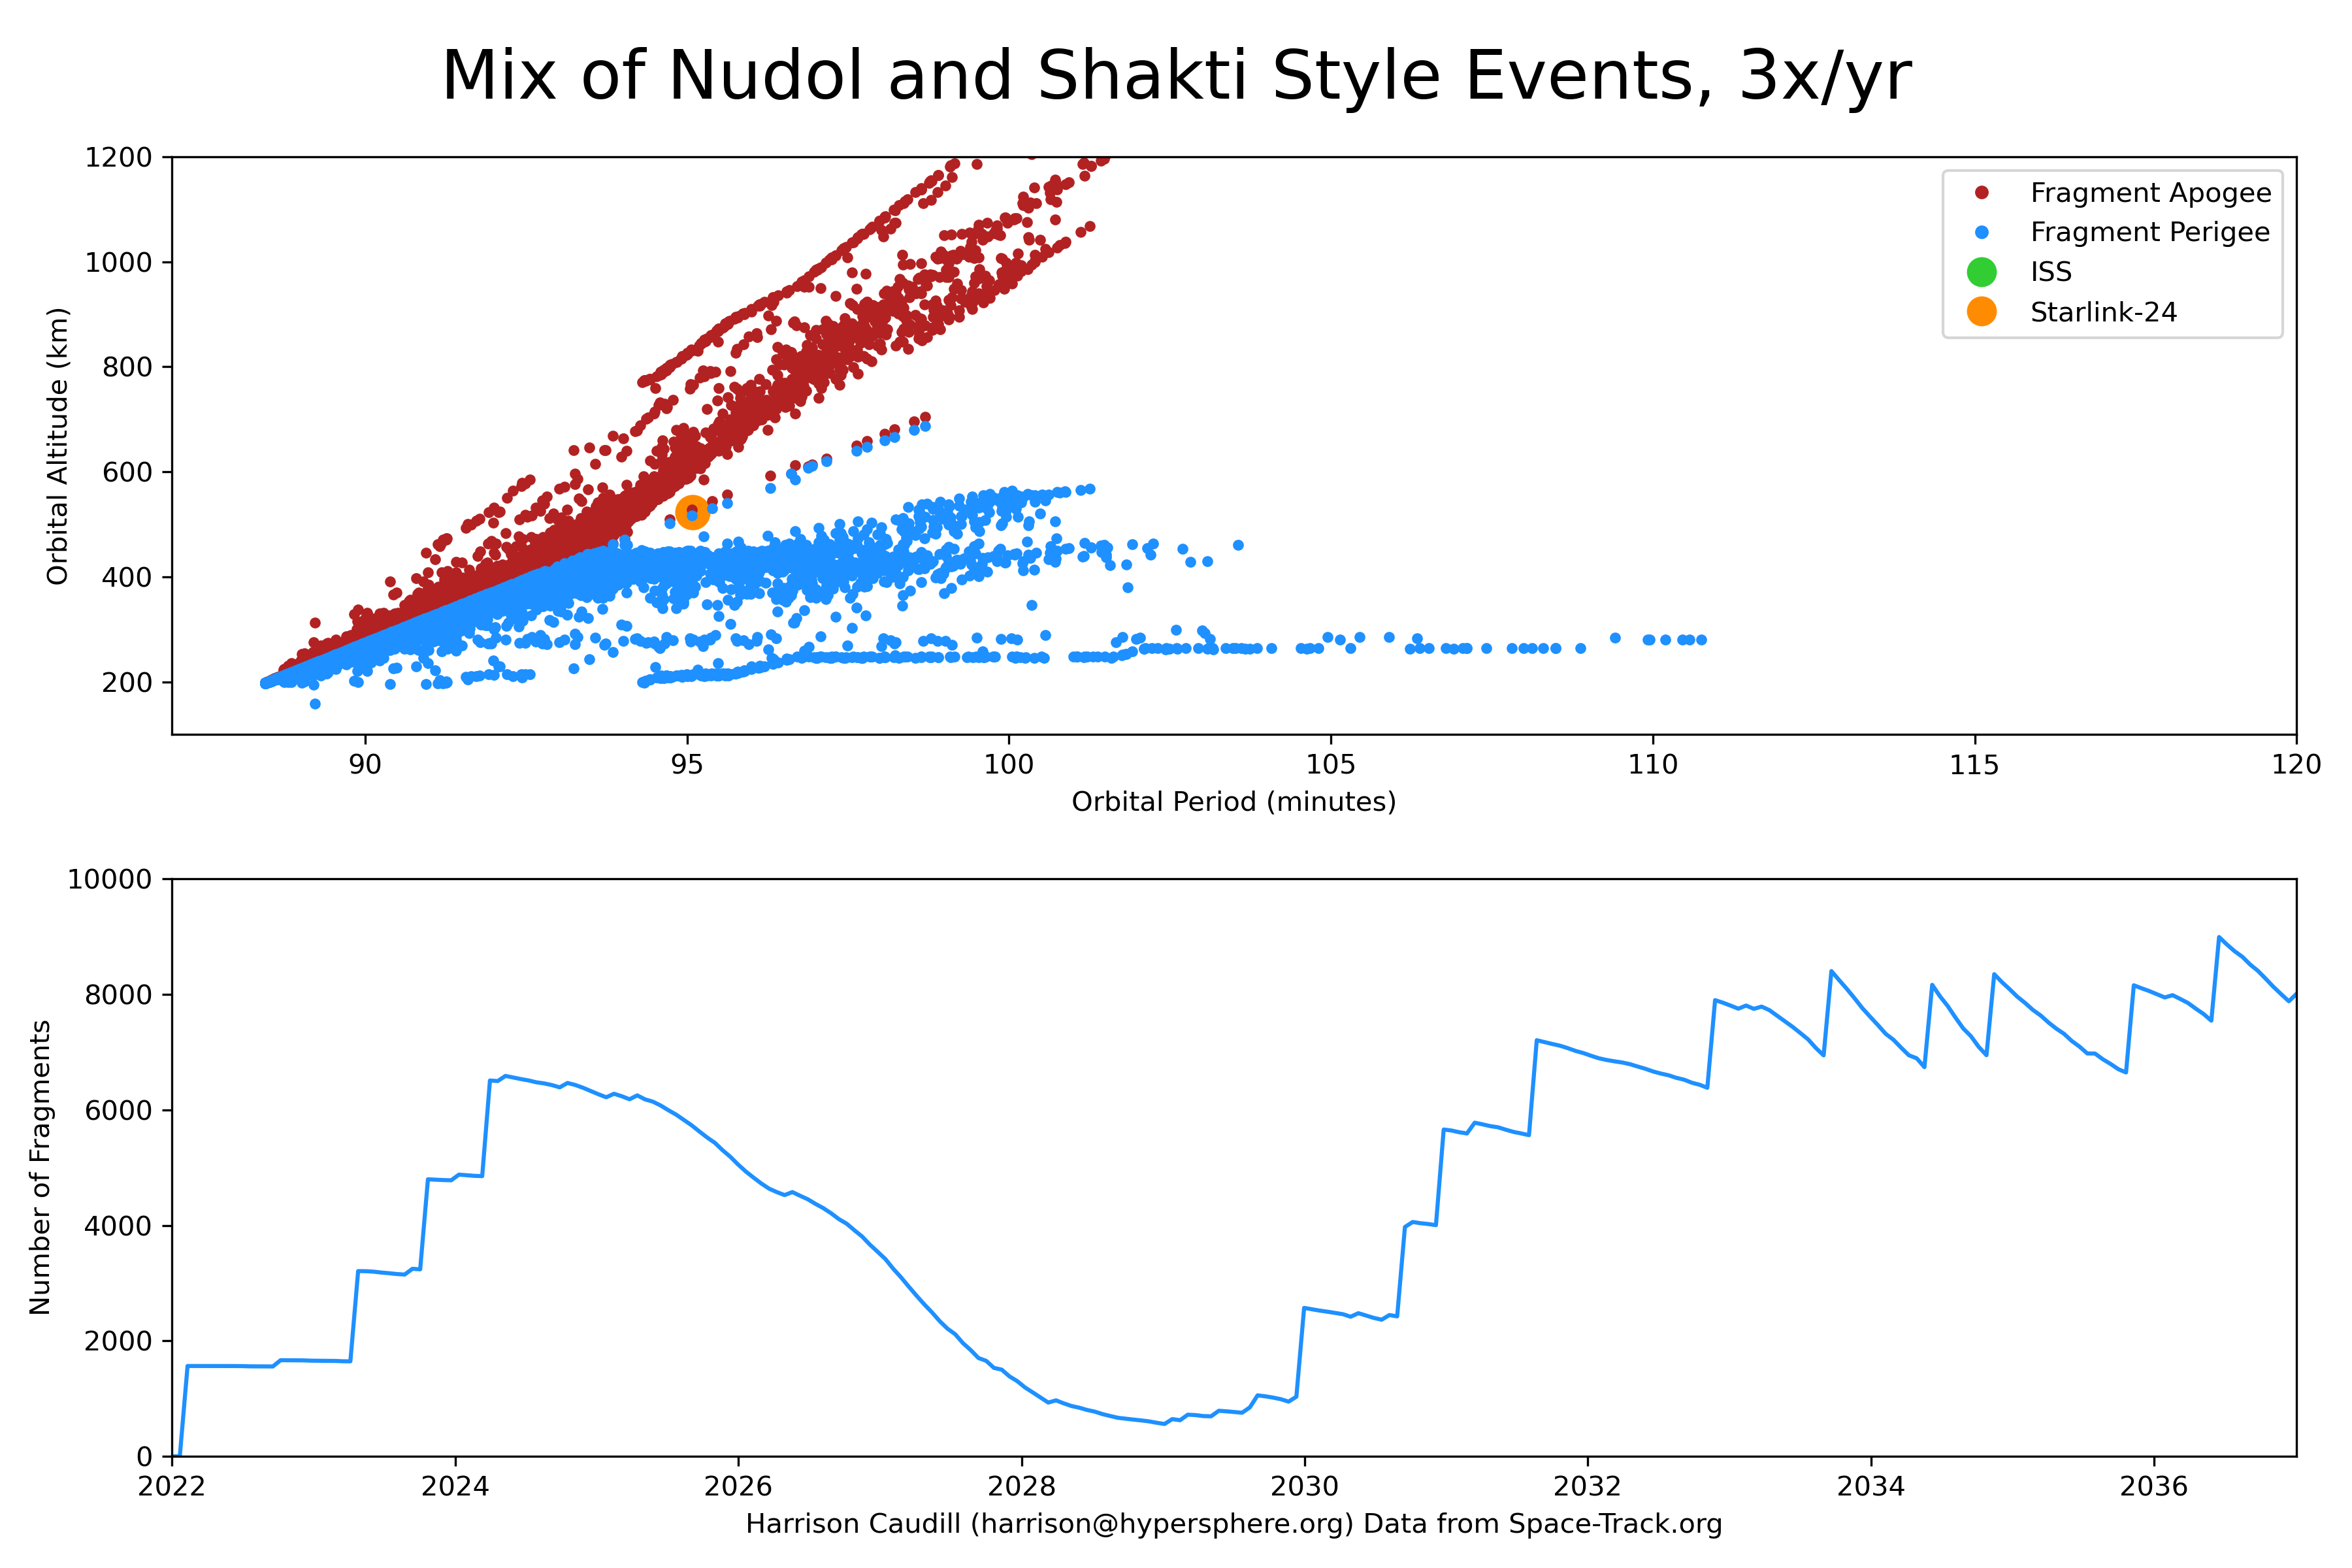
\includegraphics[width=4in]{mix.png}
  \end{center}
  \caption{Simulation of three \ac{asat} tests per year at random
    intervals.  $\frac{1}{3}$ Nudol-style events and $\frac{2}{3}$
    Shakti-style events.}
\end{figure}

\begin{figure}[h]
  % ./bin/plot -c ~/dev/nukes/gabby.cfg -n 7 -T doom -t shakti
  \label{figure::gabby::doomsday::shakti}
  \begin{center}
    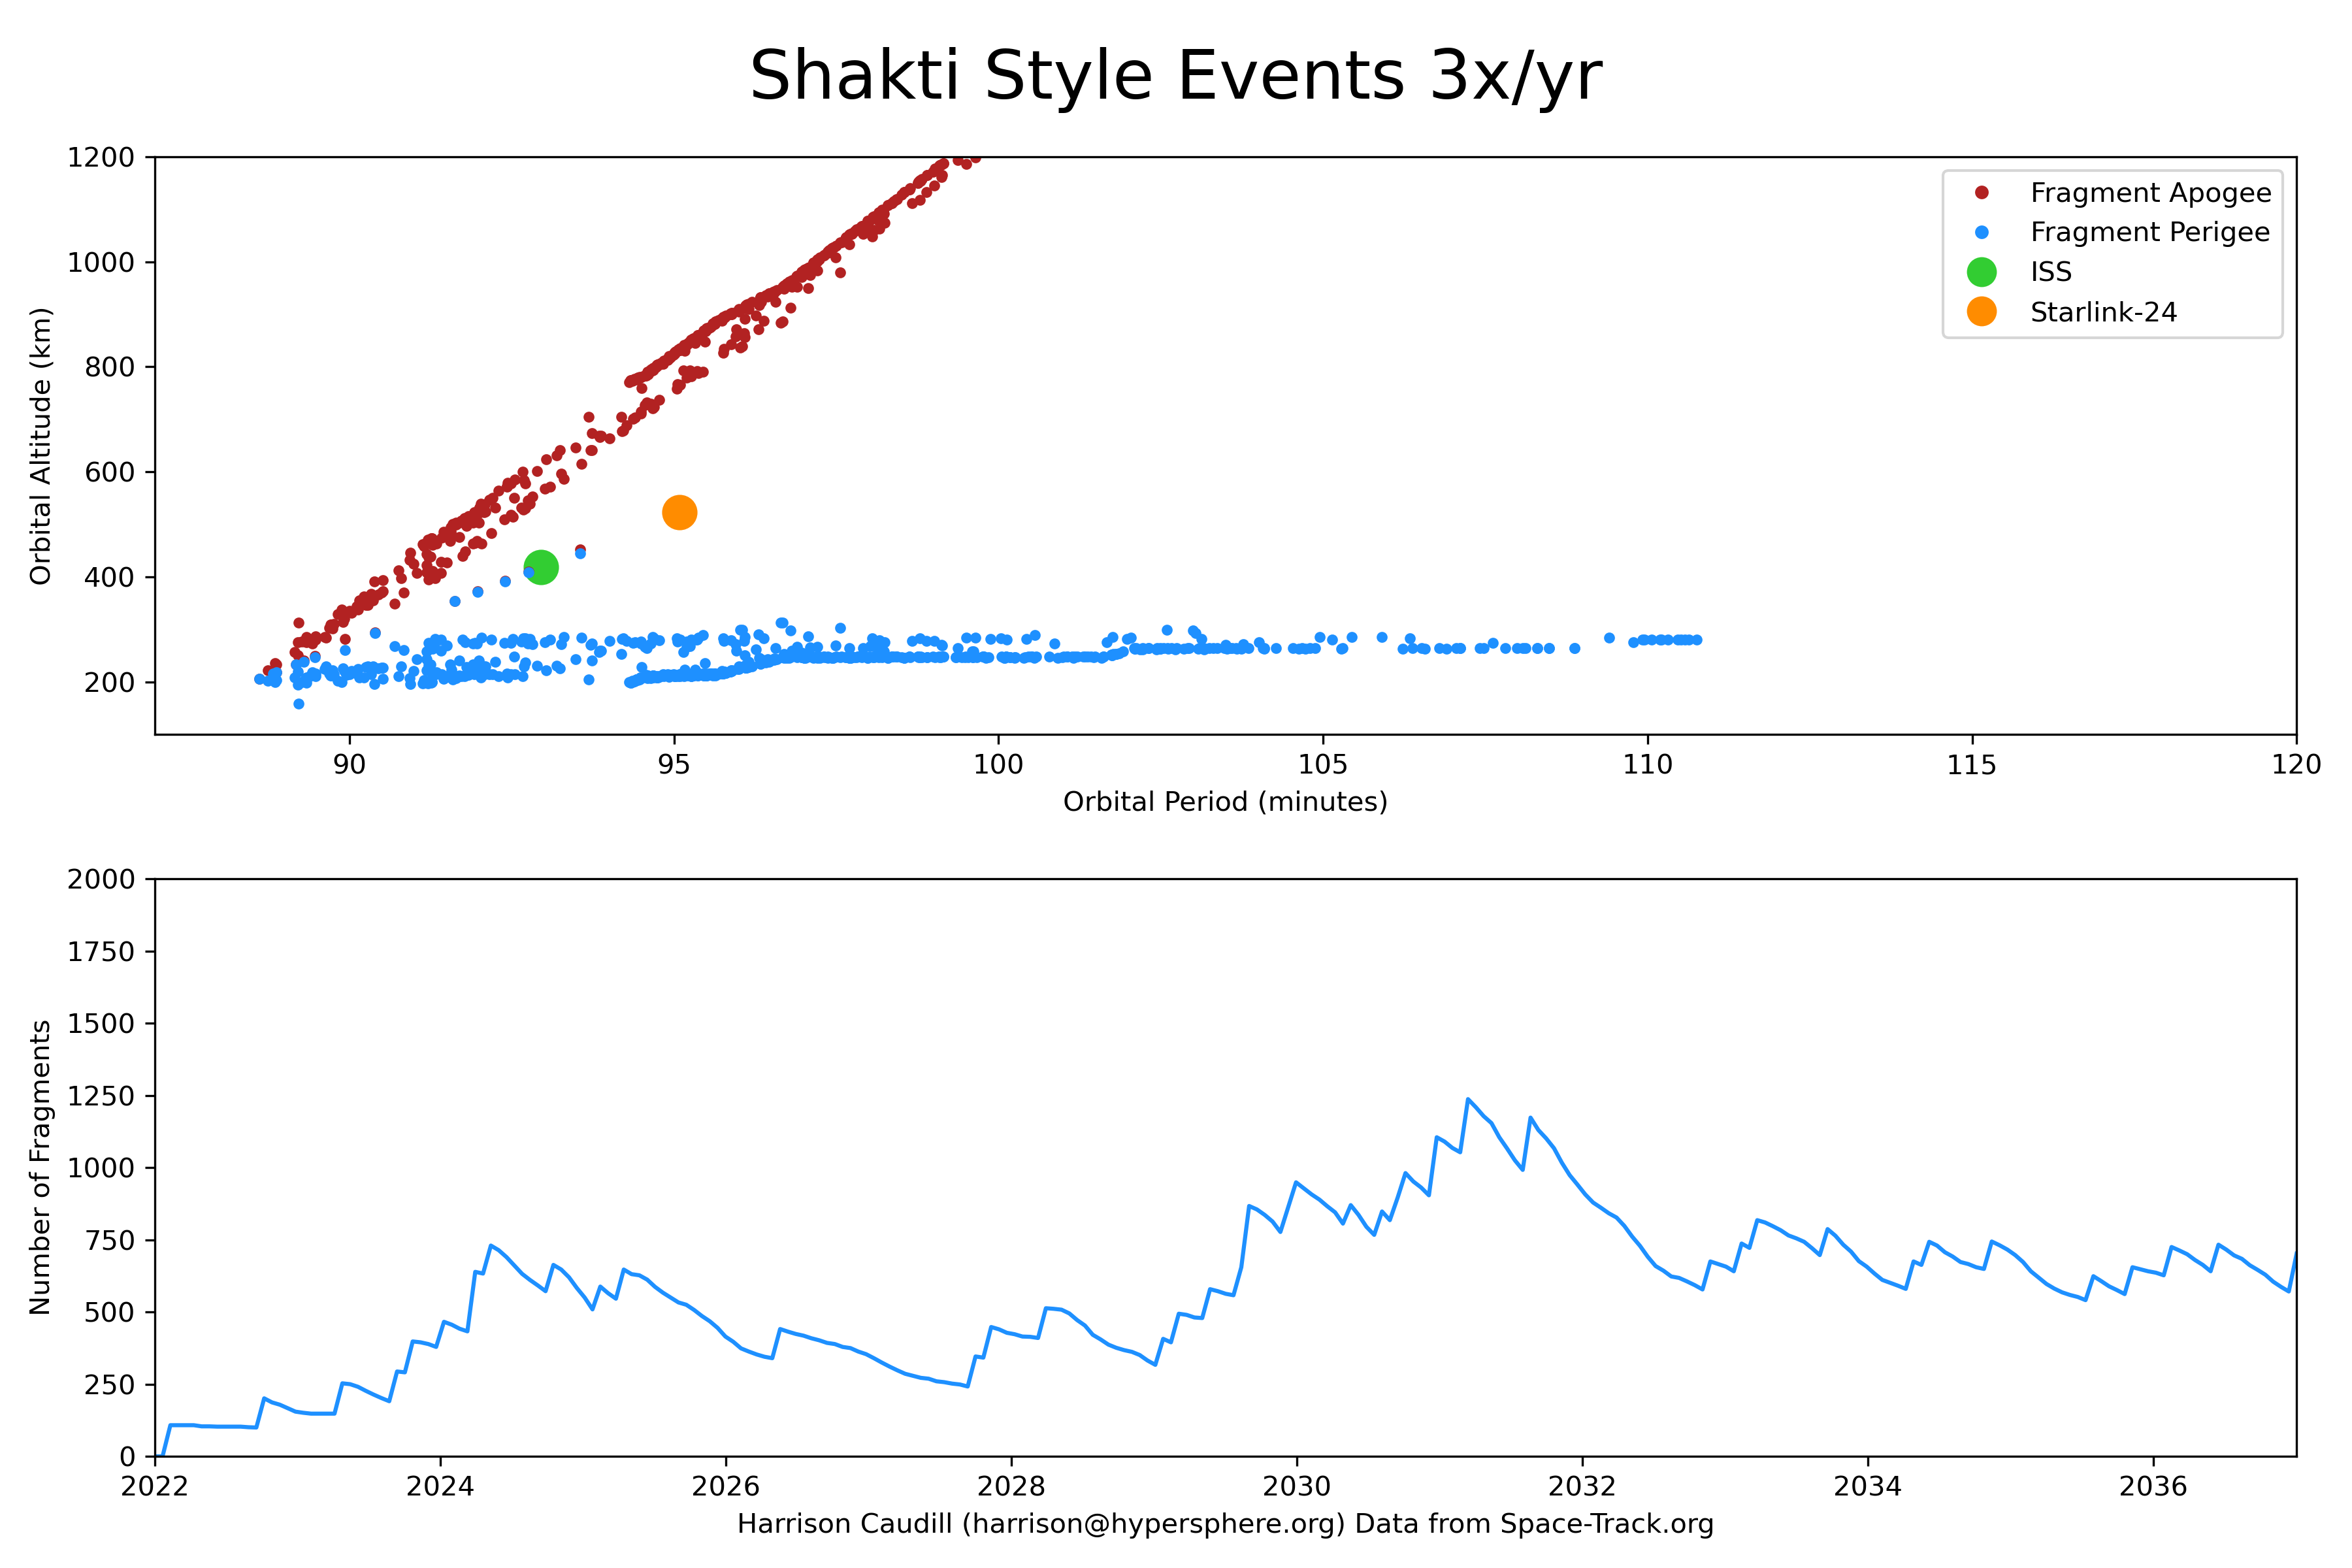
\includegraphics[width=4in]{shakti.png}
  \end{center}
  \caption{Simulation of three Shakti-style \ac{asat} tests per year
    at random intervals.}
\end{figure}
